\textbf{Ejemplo:} ?`Cu\'al es la ``probabilidad'' de que tardemos m\'as de 30 minutos en la cola del almuerzo? si sabemos que son las
13:15 de la tarde?
\begin{center}
	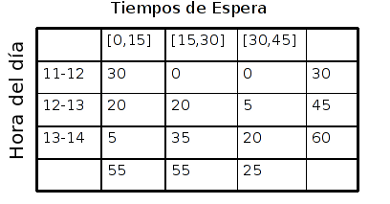
\includegraphics[height=3cm]{images/cap6_ej1_1}
\end{center}
Entonces claramente es $\frac{20}{25+55+55}\ \approx\ 14.81\%$
\subsection{Probabilidad Condicional}
\begin{itemize}
	\item Sean A,B dos sucesos tal que $P(B)>0$
	\item La probabilidad de A condicionada a la ocurrencia de B es:
	$$P(A|B)\ =\ \frac{P(A\cap B)}{P(B)}$$
	\item Notemos que la idea de frecuencias coindicionales calza perfectamente en este modelo
	\item Centra el foco de atencion en el hecho que se sabe que ha ocurrido el evento B
	\item Estamos indicando que el espacio muestral de interes se ha ``reducido'' solo a
	aquellos resultados que definen la ocurrencia del evento B
	\item Entonces $P(A|B)$ ``mide'' la probabilidad relativa de A con respecto al espacio
	reducido B
\end{itemize}
\subsection{Se respetan los axiomas basicos}
\begin{itemize}
	\item $P(A|B)\ \geq\ 0$
	\item $P(\Omega|B)\ =\ 1$
	\item Sean $A_{1},A_{2},\ldots,A_{n}$ disjuntos $A_{i}\cap A_{j}\ =\ \emptyset\ \forall i\neq j$
	$$P(\cup A_{i}|B)\ =\ \sum P(A_{i}|B)$$
\end{itemize}
\textbf{Ejemplo2:} Si lanzamos dos dados (4 caras) ?`Cu\'al es la probabilidad de que el m\'aximo
	de los resultados sea par dado que el m\'inimo de los resultados es 3?\\
	$$\Omega\ =\ {(1.1),(1.2),(1.3),\ldots,(4.4)}$$
	donde la minima es 3 $B\ =\ {(3.3),(3.4),(4.3)}$\\
	donde el maximo es par $A\ =\ {(3.4),(4.3)}$\\
	$$P(A|B)\ =\ \frac{2}{3}\ \Longleftrightarrow \frac{P(A\cap B)}{P(B)}\ =\ \frac{\frac{2}{16}}{\frac{3}{16}}\ =\ \frac{2}{3}$$
\textbf{Ejemplo3:} En una encuesta se ha determinado que los fines de semana el 45\% de la poblacion
	lee la tercera, el 35\% lee el mercurio y el 5\% lee ambos diarios. ?`Cu\'al es la probabilidad
	de que un lector de la tercera lea tambi\'en el mercurio?\\
	$$\frac{P(A\cap B)}{P(B)}\ =\ \frac{\frac{5}{100}}{\frac{45}{100}}\ =\ \frac{1}{9}$$
\textbf{Ejemplo4:} En una f\'abrica se ha recopilado la siguiente informaci\'on (expresar como probabilidades)
	\begin{itemize}
		\item El 25\% de las piezas con fallas superficiales son funcionalmente defectuosas
		\item Se sabe que el 10\% de las piezas manufacturadas tienen fallas visibles
		en la superficie
		\item Tambi\'en se ha encontrado que el 5\% de las piezas que no tenian fallas
		superficiales son funcionalmente defectuosas
	\end{itemize}
	\begin{center}
		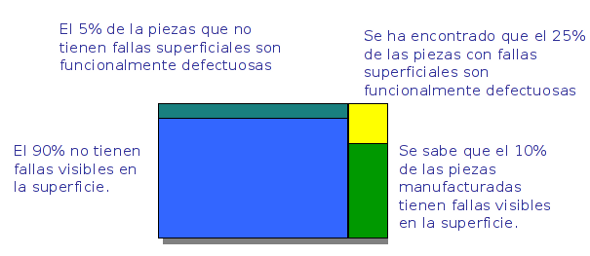
\includegraphics[height=4cm]{images/cap6_ej4_1}
	\end{center}
	B = \{ Pieza funcionalmente defectuosa \}\\
	A = \{ Pieza tiene una falla visible en la superficie \}\\
	$P(B|A)\ =\ 25\%$\\
	$P(A)\ =\ 10\%$\\
	$P(B|A^{c})\ =\ 5\%$\\
	$P(A^{c})\ =\ 90\%$\\
	$P(B)\ =\ P(B|A)P(A)\ +\ P(B|A^{c})P(A^{c})\ =\ \frac{25}{100}\cdot \frac{10}{100}\ +\ \frac{5}{100}\cdot \frac{90}{100}\ =\ \frac{7}{100}$\\
	$P(A\cap B)\ =\ P(B\cap A)\ =\ \frac{P(B|A)}{P(A)}\ =\ \frac{25}{1000}\ =\ \frac{1}{40}$\\
	$$P(A|B)\ =\ \frac{P(A\cap B)}{P(B)}\ =\ \frac{\frac{1}{40}}{\frac{7}{100}}\ =\ \frac{5}{14}$$
\subsection{Distintos Casos de la Probabilidad Condicional}
	\begin{center}
		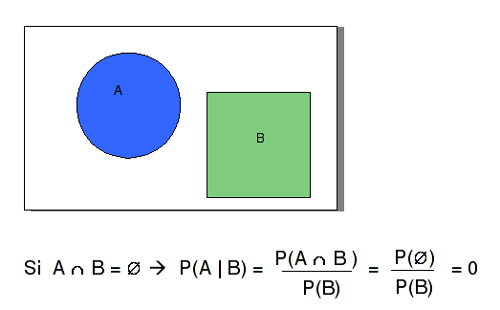
\includegraphics[height=4cm]{images/cap6_1}\\
		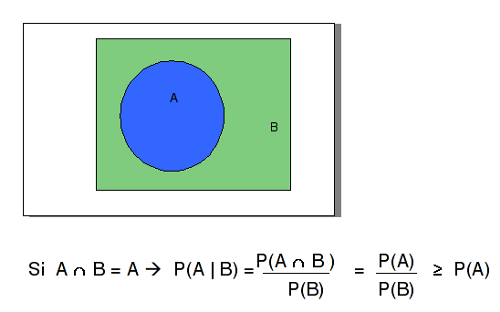
\includegraphics[height=4cm]{images/cap6_2}\\
		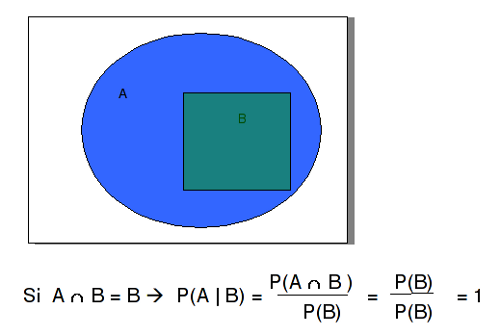
\includegraphics[height=4cm]{images/cap6_3}\\
		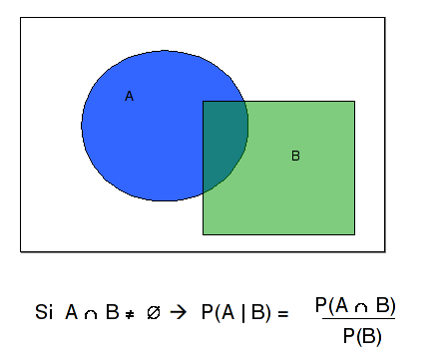
\includegraphics[height=4cm]{images/cap6_4}
	\end{center}
\subsection{Probabilidad Marginal}
	Si estudiamos la relación entre una serie de eventos $A,B,C$, llamaremos ``probabilidades
	marginales'' a las probabilidades no condicionales $P(A),\ P(B)\ y\ P(C)$. 
\subsection{Regla de Bayes}
	\begin{itemize}
		\item Sean A, B dos sucesos tal que $P(A)$, $P(B)>0$.
		\item Establece una relacion entre las probabilidades condicionales $P(A|B)$ y $P(B|A)$
		$$P(A|B)\ =\ \frac{P(B|A)P(A)}{P(B)}$$
		\item Se sigue inmediatamente de la definicion de probabilidad condicional
	\end{itemize}
\subsection{Probabilidad Total}
	Sean B1, B2,....,Bn  eventos mutuamente excluyentes tal que su uni\'on conforma
	el espacio muestral:
	$$P(\bigcup_{i=1}^{n}B_{i})\ =\ 1$$
	Entonces:
	$$P(A)\ =\ P(A|B_{1})P(B_{1})\ +\ \ldots\ +\ P(A|B_{n})P(B_{n})$$
	\begin{center}
		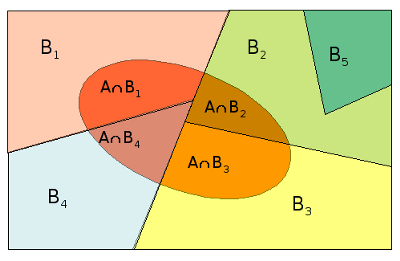
\includegraphics[height=4cm]{images/cap6_5}\\
	\end{center}
	\textbf{Ejemplo5:} Un producto se fabrica en 5 plantas que producen el 20\%, 25\%, 30\%,
	 15\% y 10\% respectivamente. Las probabilidades de fallas en cada planta est\'an dadas
	por: 0.2, 0.1, 0.15, 0.3, 0.0 ?`Cu\'al es la probabilidad de que un producto venga fallado?\\
	$P(B_1)\ =\ 20\%$\\
	$P(B_2)\ =\ 25\%$\\
	$P(B_3)\ =\ 30\%$\\
	$P(B_4)\ =\ 15\%$\\
	$P(B_5)\ =\ 10\%$\\
	$P(A)\ =\ P(A|B_{1})P(B_1)\ +\ \ldots\ +\ P(A|B_5)P(B_5)$\\
	$$P(A)\ =\ 0.2\cdot \frac{20}{100}\ +\ \ldots\ +\ 0.0\cdot \frac{10}{100}\ =\ \frac{15.5}{100}\ =\ 15.5\%$$
	\textbf{Ejemplo6:} Continuando con el anterior...supongamos de que se elige aleatoriamente
	un producto y se encuentra que est\'a fallado. ?`Cu\'al es la probabilidad que sea
	manufacturado en Planta $B_3$?\\
	$$P(B_{3}|A)\ =\ \frac{P(A|B_{3})P(B_{3})}{P(A)}\ =\ \frac{0.15\cdot \frac{30}{100}}{0.155}\ =\ 0.29\ =\ 29\%$$
\subsection{Independencia}
	\begin{itemize}
		\item Dos eventos A y B se dicen independientes ssi:
		$$P(A\cap B)\ =\ P(A)P(B) \rightarrow\ P(A|B)\ =\ P(A)\ y\ P(B|A)\ =\ P(B)$$
		\item Sean ${A_{i}:i\epsilon I={1,2,3,\ldots,k}}$ una colecci\'on de eventos de
		 $(\Omega,\xi,P)$. Se dice que los elementos son conjuntamente independientes 
		 para todo subconjunto de indices $J$:
		$$P(\bigcap_{j\epsilon J}A_{j})\ =\ \prod_{j\epsilon J}P(A_{i})$$
	\end{itemize}
	\textbf{Ejemplo7:} Sea $(\Omega,2^{\Omega},P)$ modelo de probabilidad.
		$$\Omega\ =\ {(1,0,0),(0,1,0),(0,0,1),(1,1,1)}$$
		$$P({w_{i}})\ =\ \frac{1}{4}$$
		Sean $A_{1},\ A_{2},\ A_{3}$ eventos de $(\Omega,2^{\Omega},P)$:\\
		\begin{itemize}
			\item $A_{1}:$ Primera coordenada es 1
			\item $A_{2}:$ Segunda coordenada es 1
			\item $A_{3}:$ Tercera coordenada es 1
		\end{itemize}
		$P(A_{1})\ =\ \frac{1}{2}$\\
		$P(A_{2})\ =\ \frac{1}{2}$\\
		$P(A_{3})\ =\ \frac{1}{2}$\\
		$P(A_{1}\cap A_{2})\ =\ \frac{1}{4}\ =\ P(A_{1})P(A_{2})$\\			
		$P(A_{1}\cap A_{3})\ =\ \frac{1}{4}\ =\ P(A_{1})P(A_{3})$\\			
		$P(A_{2}\cap A_{3})\ =\ \frac{1}{4}\ =\ P(A_{2})P(A_{3})$\\
		Todos son independientes (Independencia de a Pares)\\
		$P(A_{1}\cap A_{2}\cap A_{3})\ =\ \frac{1}{4}\ \neq\ P(A_{1})P(A_{2})P(A_{3})$\\
		No son independientes como Familia\\
